% !TeX root = RJwrapper.tex
\title{stplanr: A Package for Transport Planning}
\author{by Robin Lovelace, Richard Ellison}

\maketitle

\abstract{%
Tools for transport planning should be flexible, robust and scalable.
\textbf{stplanr} meets each of these criteria by providing functionality
commonly needed for transport planning in R, with an emphasis on spatial
transport data. This includes tools to import and clean transport
datasets; the creation of geographic `desire lines' from
origin-destination data; methods to assign these desire lines to the
transport network, e.g.~via interfaces to routing services such as
CycleStreets.net, Graphhopper and the OpenStreetMap Routing Machine
(OSRM); functions to calculate the geographic attributes of such routes,
such as their bearing and equidistant surroundings; and `travel
watershed' analysis. With reproducible examples and using real transport
datasets, this article demonstrates how R can form the basis of a
reproducible and flexible transport planning workflow. We conclude with
a brief discussion of desirable directions of future development.
}

\section{Introduction}\label{introduction}

The practice of transport planning can been defined as
"preparing, assessing and implementing policies, plans and projects to
improve and manage our transport systems"
\citep{jones_road_2014}.
Clearly this will involve some judgements based on intuition, experience and political considerations.
However, with the push for measurable improvements in terms of `sustainability' (e.g. reduced energy use),
the pressure on transport planners to adopt scientific methods, including computating, has grown
\citep{balmer_matsim-t:_2009}.
Transport planning is a diverse field requiring a wide range of computational tasks \citep{boyce_forecasting_2015}.
Software for transport planning should therefore be:
flexible, able to handle a wide range of data formats;
robust, able to generate reproducible results for transparent decision-making;
and scalable, able to work at multiple geographic levels from single streets to large cities and regions.

R can provide a solid basis for a transport planning workflow that meets
each of these criteria. Packages such as \CRANpkg{sp}
\citep{pebesma_classes_2005} and \CRANpkg{rgeos}
\citep{bivand_rgeos:_2016} greatly extend R's spatial data handling and
modelling capabilities \citep{bivand_applied_2013}. Packages building on
the \textbf{sp} class system have been developed for specific domains,
including \CRANpkg{SpatialEpi} \citep{kim_spatialepi:_2016},
\CRANpkg{diseasemapping} \citep{brown_diseasemapping:_2016} and the
\textbf{adehabitat} family of packages \citep{calenge_package_2006}.

Inspired by such efforts and driven by our own research needs, our
primary aim for \textbf{stplanr} is to provide an R toolbox for
transport planning. Although the focus is on spatial transport datasets
(and most transport problems contain a spatial component),
\textbf{stplanr} also provides functions for handling non-spatial
datasets.

\subsection{Motivations}\label{motivations}

There has been little in the way of R development for transport
applications. This is surprising given the ubiquity of transport
problems,\footnote{Most people can identify interventions that they
  think would make the transport systems they interact with more
  sustainable. Think about the paths and roads you travel on, for
  example: what interventions would you prioritise to improve
  non-motorised access, for walking, cycling and wheel-chairs? What
  quantitative evidence would you need to communicate this to the
  relevant authorities?} R's aptitude for handling transport data
(including spatial and travel survey data), and the increasing use of R
in applied domains. Increasingly, R is the go-to statistical software in
many organisations: academic, public sector and privately owned. Such
organisations undertake the majority of transport planning research.
This paper was therefore motivated by the desire to demonstrate that R
provides an excellent framework for transport research. If readers
decide not to use the package, perhaps needing bespoke solutions to
specific transport problems not covered by \textbf{stplanr}, it is hoped
that the ideas, functions and datasets described in this paper inspire
parallel developments in the space of `R for transport applications'.
Moreover, by making the package deliberately broad in its scope, we hope
that \textbf{stplanr} can help build a nascent community of R-using
transport researchers. We welcome feature requests and feedback at the
package's \href{https://github.com/ropensci/stplanr/issues}{online
home}.

R is already used in transport applications, as illustrated by recent
research that applies packages from other domains to transport problems.
For instance, \citeauthor{efthymiou_use_2012}
(\citeyear{efthymiou_use_2012}) use R to analyse the data collected from
an online survey focused on car-sharing, bicycle-sharing and electric
vehicles. \citeauthor{efthymiou_use_2012}
(\citeyear{efthymiou_use_2012}) also used R to collect and analyse
transport-related data from Twitter using packages including
\CRANpkg{XML}, \CRANpkg{twitteR} and \CRANpkg{ggplot2}. These packages
were used to download, parse and plot the Twitter data using a method
that can be repeated and the results reproduced or updated. More general
statistical analyses have also been conducted on transport-related
datasets using packages including \CRANpkg{muStat} and \CRANpkg{mgcv}
\citep{diana_studying_2012,cerin_walking_2013}. Despite the rising use
of R for transport research, there has yet been to be a package for
transport planning.

The design of the R language, with its emphasis on flexibility, data
processing and statistical modelling, suggests it can provide a powerful
environment for transport planning research. There are many quantitative
methods in transport planning \citep{ortuzar_modelling_2001} and we have
attempted to focus on those that are most generalisable and frequently
used. \textbf{stplanr} facilitates the following common computational
tasks for transport planning:

\begin{itemize}
\tightlist
\item
  Accessing and processing of data on transport infrastructure and
  behaviour
\item
  Analysis and visualisation of the transport network
\item
  Analysis of origin-destination (OD) data and the visualisation of
  resulting `desire lines'
\item
  The allocation of desire lines to roads and other guideways via
  routing algorithms to show commonly used routes through geographical
  space
\item
  The aggregation of routes to estimate total levels of flow on segments
  throughout the transport network
\item
  Development of models to estimate transport behaviour currently and
  under various scenarios of change
\item
  The calculation of `catchment areas' affected by transport
  infrastructure
\end{itemize}

The automation of such tasks can assist researchers and practitioners to
create evidence for decision making. If the data processing and analysis
stages are fast and painless, more time can be dedicated to
visualisation and decision making. This should allow researchers to
focus on problems, rather than on wrestling with unwieldy datasets,
clunky graphical user interfaces (GUIs), and ad-hoc scripts that could
be generalised. Furthermore, if the process can be made reproducible and
accessible (e.g.~via online visualisation packages such as
\CRANpkg{shiny} and \CRANpkg{leaflet}), this will help transport
planning move away from reliance on `black boxes' and become a more
transparent and democratic activity
\citep{waddell_urbansim:_2002,hollander_who_2015}.

The technical advantages of using modern, interpreted, and open source
languages such as R are manifold: they enable automation and sharing of
methods between researchers, for example the application of methods
developed for one city to another; they ease the integration with other
software systems and the web; and they have very strong user
communities. The advantages of using R specifically to develop the
functionality described in this paper are that it has unparalleled
geo-statistical capabilities \citep{pebesma_software_2015},
visualisation packages (e.g. \CRANpkg{tmap}, \CRANpkg{ggplot2}) and the
ability to rapidly read-in data stored in many formats (e.g.~via the
\CRANpkg{haven} and \CRANpkg{rio} packages).

\section{Package structure and
functionality}\label{package-structure-and-functionality}

The package can be installed and loaded in the usual way (see the
package's \href{https://github.com/ropensci/stplanr}{README} for
dependencies and access to development versions):

\begin{Schunk}
\begin{Sinput}
install.packages("stplanr")
\end{Sinput}
\end{Schunk}

\begin{Schunk}
\begin{Sinput}
library(stplanr)
\end{Sinput}
\begin{Soutput}
#> Loading required package: sp
\end{Soutput}
\end{Schunk}

As illustrated by the message emitted when \textbf{stplanr} is loaded,
it depends on \CRANpkg{sp}. This means that the spatial data classes
commonly used in the package will work with generic R functions such as
\texttt{summary}, \texttt{aggregate} and, as illustrated in the figures
below, \texttt{plot} \citep{bivand_applied_2013}.

\subsection{Core functions and
classes}\label{core-functions-and-classes}

The package's core functions are structured around 3 common types of
spatial transport data:

\begin{itemize}
\tightlist
\item
  Origin-destination (OD) data, which report the number of people
  travelling between origin-destination pairs. This type of data is not
  explicitly spatial (OD datasets are usually represented as data
  frames) but represents movement over space between points in
  geographical space. An example is provided in the \texttt{flow}
  dataset.
\item
  Line data, one dimensional linear features on the surface of the
  Earth. These are typically stored as a \texttt{SpatialLinesDataFrame}.
\item
  Route data are special types of lines which have been allocated to the
  transport network. Routes typically result from the allocation of a
  straight `desire line' allocated to the route network with a
  \texttt{route\_} function. Route network represent many overlapping
  routes. All are typically stored as \texttt{SpatialLinesDataFrame}.
\end{itemize}

For ease of use, functions focussed on each data type have been
developed with names prefixed with \texttt{od\_}, \texttt{line\_} and
\texttt{route\_} respectively. A selection of these is presented in
Table 1. Additional `core functions' could be developed, such as those
prefixed with \texttt{rn\_} (for working with route network data) and
\texttt{g\_} functions for geographic operations such as buffer creation
on lat/lon projected data (this function is currently named
\texttt{buff\_geo}). We plan to elicit feedback on such changes before
implementing them.

\begin{longtable}[]{@{}lll@{}}
\caption{Selection of functions for working with or generating OD, line
and route data types.}\tabularnewline
\toprule
Function & Input data type(s) & Output data type\tabularnewline
\midrule
\endfirsthead
\toprule
Function & Input data type(s) & Output data type\tabularnewline
\midrule
\endhead
od\_dist & Data frame & Numeric vector\tabularnewline
od\_id\_order & Data frame & Data frame\tabularnewline
line\_bearing & Spatial line & Numeric vector\tabularnewline
line\_midpoint & Spatial line & Spatial points\tabularnewline
route\_cyclestreet & Coordinates, spatial point or text & Spatial
lines\tabularnewline
route\_graphhopper & Coordinates, spatial point or text & Spatial
lines\tabularnewline
\bottomrule
\end{longtable}

With a tip of the hat to the concept of type stability (e.g.~as
implemented in \CRANpkg{dplyr}), we also plan to make the core functions
of \textbf{stplanr} more type-stable in future releases. Core functions,
which begin with the prefixes listed above, could follow
\CRANpkg{dplyr}'s lead and return only objects with the same class as
that of the input. However there are limitations to this approach: it
will break existing functionality and mean that output objects have a
larger size than necessary (\texttt{line\_bearing}, for example, does
not need to duplicate the spatial data contained in its input). Instead,
we plan to continue to name functions around the type of \emph{input}
data they take, but are open minded about function input-output data
class conventions, especially in the context of the new class system
implemented in \CRANpkg{sf}.

A class system has not been developed for each data type (this option is
discussed in the final section). The most common data types used in
\textbf{stplanr} are assumed to be data frames and spatial datasets.

Transport datasets are very diverse. There are therefore many other
functions which have more ad-hock names. Rather attempt a systematic
description of each of \textbf{stplanr}'s functions (which can be
gleaned from the online manual) it is more illuminating to see how they
work together, as part of a transport planning workflow. As with most
workflows, this begins with data access and ends with visualisation.

\subsection{Accessing and processing transport
data}\label{accessing-and-processing-transport-data}

Gaining access to data is often the first stage in transport research.
This is often a long and protracted process which is thankfully becoming
easier thanks to the `open data' movement and packages such as
\textbf{tigris} for making data access from within R easier
\citep{walker_tigris:_2016}.

\textbf{stplanr} provides a variety of different functions that
facilitate importing common data formats used for transport analysis
into R. Although transport analysis generally requires some
transport-specific datasets, it also typically relies heavily on common
sources of data including census data. This being the case,
\textbf{stplanr} also includes functions that may be useful to those not
involved in transport research. This includes the
\texttt{read\_table\_builder} function for importing data from the
Australian Bureau of Statistics (ABS) and the UK's Stats19 road traffic
casualty dataset. A brief example of the latter is demonstrated below,
which begins with downloading the data (warning this downloads
\textasciitilde{}100 MB of data):

\begin{Schunk}
\begin{Sinput}
dl_stats19() # download and extract stats19 road traffic casualty data
\end{Sinput}
\end{Schunk}

\begin{verbatim}
#> [1] "Data saved at: /tmp/RtmpppF3E2/Accidents0514.csv"
#> [2] "Data saved at: /tmp/RtmpppF3E2/Casualties0514.csv"
#> [3] "Data saved at: /tmp/RtmpppF3E2/Vehicles0514.csv"
\end{verbatim}

Once the data has been saved in the default directory, determined by
\texttt{tempdir()}, it can be read-in and cleaned with the
\texttt{read\_stats19\_} functions (note these call
\texttt{format\_stats19\_} functions internally to clean the datasets
and add correct labels to the variables):

\begin{Schunk}
\begin{Sinput}
ac <- read_stats19_ac()
ca <- read_stats19_ca()
ve <- read_stats19_ve()
\end{Sinput}
\end{Schunk}

The resulting datasets (representing accident, casualty and vehicle
level data, respectively) can be merged and made geographic, as
illustrated below:

\begin{Schunk}
\begin{Sinput}
library(dplyr)
ca_ac <- inner_join(ca, ac)
ca_cycle <- ca_ac %>%
  filter(Casualty_Severity == "Fatal" & !is.na(Latitude)) %>%
  select(Age = Age_of_Casualty, Mode = Casualty_Type, Longitude, Latitude)
ca_sp <- SpatialPointsDataFrame(coords = ca_cycle[3:4], data = ca_cycle[1:2])
\end{Sinput}
\end{Schunk}

Now that this casualty data has been cleaned, subsetted (to only include
serious cycle crashes) and converted into a spatial class system, we can
analyse them using geographical datasets of the type commonly used by
\textbf{stplanr}. The following code, for example, geographically
subsets the dataset to include only crashes that occured within the
bounding box of a
\href{https://github.com/ropensci/stplanr/blob/master/data/route_network.rda?raw=true}{route
network dataset} provided by \textbf{stplanr} (from version 0.1.7 and
beyond) using the function \texttt{bb2poly}, which converts a spatial
dataset into a box, represented as a rectangular
\texttt{SpatialPolygonsDataFrame}:

\begin{Schunk}
\begin{Sinput}
data("route_network") # devtools::install_github("ropensci/splanr")version 0.1.7
proj4string(ca_sp) <- proj4string(route_network)
bb <- bb2poly(route_network)
proj4string(bb) <- proj4string(route_network)
ca_local <- ca_sp[bb,]
\end{Sinput}
\end{Schunk}

The above code chunk shows the importance of understanding geographical
data when working with transport data. It is only by converting the
casualty data into a spatial data class, and adding a coordinate
reference system (CRS), that transport planners and researchers can link
this important dataset back to the route network. We can now perform GIS
operations on the results. The next code chunk, for example, finds all
the fatalities that took place within 100 m of the route network, using
the function \texttt{buff\_geo}:

\begin{Schunk}
\begin{Sinput}
rnet_buff_100 <- buff_geo(route_network, width = 100)
ca_buff <- ca_local[rnet_buff_100,]
\end{Sinput}
\end{Schunk}

These can be visualised using base R graphics, extended by \CRANpkg{sp},
as illustrated in Figure \ref{fig:fats}. This provides a good start for
analysis but for publication-quality plots and interactive plots,
designed for public engagement, we recommend using dedicated
visualisation packages that work with spatial data such as
\CRANpkg{tmap}.

\begin{Schunk}
\begin{Sinput}
plot(bb, lty = 4)
plot(rnet_buff_100, col = "grey", add = TRUE)
points(ca_local, pch = 4)
points(ca_buff, cex = 3)
\end{Sinput}
\begin{figure}

{\centering 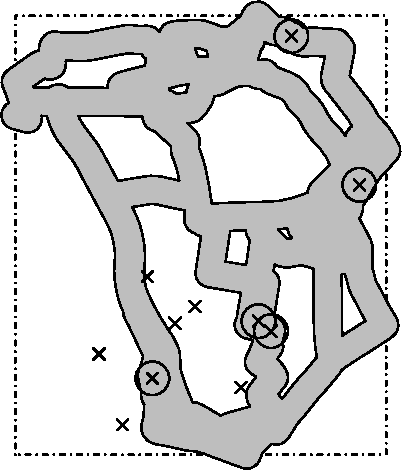
\includegraphics[width=0.5\linewidth]{fats-1}

}

\caption[Road traffic fatalities in the study area downloaded with with stplanr (crosses)]{Road traffic fatalities in the study area downloaded with with stplanr (crosses). Deaths that happened within 100 m of the route network are represented by circles.}\label{fig:fats}
\end{figure}
\end{Schunk}

\subsection{Creating geographic desire
lines}\label{creating-geographic-desire-lines}

Perhaps the most common type of aggregate-level transport information is
origin-destination (`OD') data. This can be presented either as a matrix
or (more commonly) a long table of OD pairs. An example of this type of
raw data is provided below (see \texttt{?flow} to see how this dataset
was created).

\begin{Schunk}
\begin{Sinput}
data("flow", package = "stplanr")
head(flow[c(1:3, 12)])
\end{Sinput}
\begin{Soutput}
#>        Area.of.residence Area.of.workplace All Bicycle
#> 920573         E02002361         E02002361 109       2
#> 920575         E02002361         E02002363  38       0
#> 920578         E02002361         E02002367  10       0
#> 920582         E02002361         E02002371  44       3
#> 920587         E02002361         E02002377  34       0
#> 920591         E02002361         E02002382   7       0
\end{Soutput}
\end{Schunk}

Although the flow data displayed above describes movement over
geographical space, it contains no explicitly geographical information.
Instead, the coordinates of the origins and destinations are linked to a
separate geographical dataset which also must be loaded to analyse the
flows. This is a common problem solved by the function \texttt{od2line}.
The geographical data is a set of points representing centroids of the
origin and destinations, saved as a \texttt{SpatialPointsDataFrame}.
Geographical data in R is best represented as such \texttt{Spatial*}
objects, which use the \texttt{S4} object engine. This explains the
close integration of \textbf{stplanr} with R's spatial packages,
especially \textbf{sp}, which defines the \texttt{S4} spatial object
system.

\begin{Schunk}
\begin{Sinput}
data("cents", package = "stplanr")
as.data.frame(cents[1:3, -c(3,4)])
\end{Sinput}
\begin{Soutput}
#>       geo_code  MSOA11NM coords.x1 coords.x2
#> 1708 E02002384 Leeds 055 -1.546463  53.80952
#> 1712 E02002382 Leeds 053 -1.511861  53.81161
#> 1805 E02002393 Leeds 064 -1.524205  53.80410
\end{Soutput}
\end{Schunk}

We use \texttt{od2line} to combine \texttt{flow} and \texttt{cents}, to
join the former to the latter. We will visualise the \texttt{l} object
created below in the next section.

\begin{Schunk}
\begin{Sinput}
l <- od2line(flow = flow, zones = cents)
\end{Sinput}
\end{Schunk}

The data is now in a form that is much easier to analyse. We can plot
the data with the command \texttt{plot(l)}, which was not possible
before. Because the \texttt{SpatialLinesDataFrame} object also contains
data per line, it also helps with visualisation of the flows, as
illustrated in Figure \ref{fig:lines_routes}.

\subsection{Allocating flows to the transport
network}\label{allocating-flows-to-the-transport-network}

A common problem faced by transport researchers is network allocation:
converting the `as the crow flies' lines illustrated in the figure above
into routes. These are the complex, winding paths that people and
animals make to avoid obstacles such as buildings and to make the
journey faster and more efficient (e.g.~by following the route network).

This is difficult (and was until recently near impossible using free
software) because of the size and complexity of transport networks, the
complexity of realistic routing algorithms and need for
context-specificity in the routing engine. Inexperienced cyclists, for
example, would take a very different route than a heavy goods vehicle.
\textbf{stplanr} tackles this issue by using 3rd party APIs to provide
route-allocation.

Route allocation is undertaken by \code{route\_} functions such as
\code{route\_cyclestreets} and \linebreak \code{route\_graphhopper}.
These allocate a single OD pair, represented as a text string to be
`geo-coded', a pair of of coordinates, or two \texttt{SpatialPoints}
objects, representing origins and destinations. This is illustrated
below with \texttt{route\_cyclestreet}, which uses the
\href{http://www.cyclestreets.net/api/}{CycleStreets.net API}, a routing
service ``by cyclists for cyclists'' that offers a range route
strategies (primarily `fastest', `quietest' and `balanced') that are
based on a detailed analysis of cyclist wayfinding:\footnote{An API key
  is needed for this function to work. This can be requested (or
  purchased for large scale routing) from
  \href{https://www.cyclestreets.net/api/apply/}{cyclestreets.net/api/apply}.
  See \texttt{?route\_cyclestreet} for details. Thanks to Martin
  Lucas-Smith and Simon Nuttall for making this possible.}

\begin{Schunk}
\begin{Sinput}
route_bl <- route_cyclestreet(from = "Bradford", to = "Leeds")
route_c1_c2 <- route_cyclestreet(cents[1,], cents[2,])
\end{Sinput}
\end{Schunk}

The raw output from routing APIs is usually provided as a JSON or
GeoJSON text string. By default, \texttt{route\_cyclestreet} saves a
number of key variables (including length, time, hilliness and busyness
variables generated by CycleStreets.net) from the attribute data
provided by the API. If the user wants to save the raw output, the
\texttt{save\_raw} argument can be used:

\begin{Schunk}
\begin{Sinput}
route_bl_raw <- route_cyclestreet(from = "Bradford", to = "Leeds", save_raw = TRUE)
\end{Sinput}
\end{Schunk}

Additional arguments taken by the \texttt{route\_} functions depend on
the routing function in question. By changing the \texttt{plan} argument
of \texttt{route\_cyclestreet} to \texttt{fastest}, \texttt{quietest} or
\texttt{balanced}, for example, routes favouring speed, quietness or a
balance between speed and quietness will be saved, respectively.

To automate the creation of route-allocated lines over many desire
lines, the \texttt{line2route} function loops over each line, wrapping
any \texttt{route\_} function as an input. The output is a
\texttt{SpatialLinesDataFrame} with the same number of dimensions as the
input dataset (see the right panel in Figure \ref{fig:lines_routes}).

\begin{verbatim}
routes_fast <- line2route(l = l, route_fun = route_cyclestreet)
\end{verbatim}

The result of this `batch routing' exercise is illustrated in Figure
\ref{fig:lines_routes}. The red lines in the left hand panel are very
different from the hypothetical straight `desire lines' often used in
transport research, highlighting the importance of this route-allocation
functionality.

\begin{Schunk}
\begin{Sinput}
plot(route_network, lwd=0)
plot(l, lwd = l$All / 10, add = TRUE)
lines(routes_fast, col = "red")
routes_fast$All <- l$All
rnet <- overline(routes_fast, "All", fun = sum)
rnet$flow <- rnet$All / mean(rnet$All) * 3
plot(rnet, lwd = rnet$flow / mean(rnet$flow))
\end{Sinput}
\begin{figure}
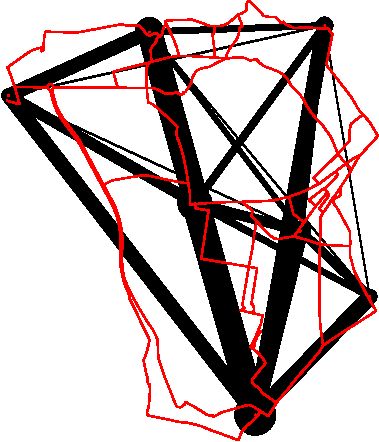
\includegraphics[width=0.5\linewidth]{lines_routes-1} 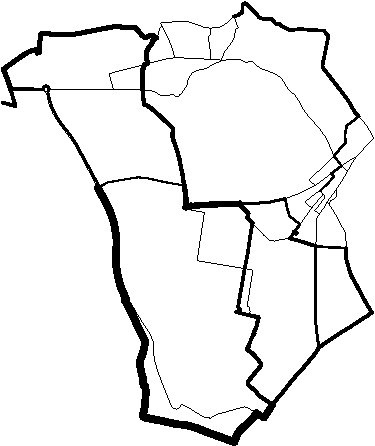
\includegraphics[width=0.5\linewidth]{lines_routes-2} \caption[Visualisation of travel desire lines, with width proportional to number of trips between origin and destination (black) and routes allocated to network  (red) in the left-hand panel]{Visualisation of travel desire lines, with width proportional to number of trips between origin and destination (black) and routes allocated to network  (red) in the left-hand panel. The right hand panel shows the route network dataset generated by overline().}\label{fig:lines_routes}
\end{figure}
\end{Schunk}

To estimate the amount of capacity needed at each segment on the
transport network, the \texttt{overline} function demonstrated above, is
used to divide line geometries into unique segments and aggregate the
overlapping values. The results, illustrated in the right-hand panel of
Figure \ref{fig:lines_routes}, can be used to estimate where there is
most need to improve the transport network, for example informing the
decision of where to build new bicycle paths.

Limitations with the \texttt{route\_cyclestreet} routing API include its
specificity, to one mode (cycling) and a single region (the UK and part
of Europe). To overcome these limitations, additional routing APIs were
added with the functions \texttt{route\_graphhopper},
\texttt{route\_transportapi\_public} and \texttt{viaroute}. These
interface to Graphhopper, TransportAPI and the Open Source Routing
Machine (OSRM) routing services, respectively. The great advantage of
OSRM is that it allows you to run your own routing services on a local
server, greatly increasing the rate of route generation.

A short example of finding the route by car and bike between New York
and Oaxaca demonstrates how \texttt{route\_graphhopper} can collect
geographical and other data on routes by various modes, anywhere in the
world. The output, shown in Table \ref{tab:xtnyoa}, shows that the
function also saves time, distance and (for bike trips) vertical
distance climbed for the trips.

\begin{Schunk}
\begin{Sinput}
ny2oaxaca1 <- route_graphhopper("New York", "Oaxaca", vehicle = "bike")
ny2oaxaca2 <- route_graphhopper("New York", "Oaxaca", vehicle = "car")
rbind(ny2oaxaca1@data, ny2oaxaca2@data)
\end{Sinput}
\end{Schunk}

\begin{longtable}[]{@{}rrr@{}}
\toprule
time & dist & change\_elev\tabularnewline
\midrule
\endhead
17522.73 & 4885663 & 87388.13\tabularnewline
2759.89 & 4754772 & NA\tabularnewline
\bottomrule
\end{longtable}

\subsection{Modelling travel catchment
areas}\label{modelling-travel-catchment-areas}

Accessibility to transport services is a particularly important topic
when considering public transport or active travel because of the
frequent steep reduction in use as distances to access services (or
infrastructure) increase. As a result, the planning for transport
services and infrastructure frequently focuses on several measures of
accessibility including distance, but also travel times and frequencies
and weighted by population. The functions in \textbf{stplanr} are
intended to provide a method of estimating these accessibility measures
as well as calculating the population that can access specific services
(i.e., estimating the catchment area).

Catchment areas in particular are a widely used measure of accessibility
that attempts to both quantify the likely target group for a particular
service, and visualise the geographic area that is covered by the
service. For instance, passengers are often said to be willing to walk
up to 400 metres to a bus stop, or 800 metres to a railway station
\citep{el-geneidy_new_2014}. Although these distances may appear
relatively arbitrary and have been found to underestimate the true
catchment area of bus stops and railway stations
\citep{el-geneidy_new_2014,daniels_explaining_2013} they nonetheless
represent a good, albeit somewhat conservative, starting point from
which catchment areas can be determined.

In many cases, catchment areas are calculated on the basis of
straight-line (or ``as the crow flies'') distances. This is a
simplistic, but relatively appealing approach because it requires little
additional data and is straight-forward to understand. \textbf{stplanr}
provides functionality that calculates catchment areas using
straight-line distances with the \texttt{calc\_catchment} function. This
function takes a \texttt{SpatialPolygonsDataFrame} that contains the
population (or other) data, typically from a census, and a
\texttt{Spatial*} layer that contains the geometry of the transport
facility. These two layers are overlayed to calculate statistics for the
desired catchments including proportioning polygons to account for the
proportion located within the catchment area.

To illustrate how catchment areas can be calculated, \textbf{stplanr}
contains some sample datasets stored in ESRI Shapefile format (a
commonly used format for distributing GIS layers) that can together be
used to calculate sample catchment areas. One of these datasets
(\texttt{smallsa1}) contains population data for Statistical Area 1
(SA1) zones in Sydney, Australia. The second contains hypothetical
cycleways aligned to streets in Sydney. The code below unzips the
datasets and reads in the shapefiles using the \texttt{readOGR} function
of \CRANpkg{rgdal}.

\begin{Schunk}
\begin{Sinput}
data_dir <- system.file("extdata", package = "stplanr")
unzip(file.path(data_dir, 'smallsa1.zip'))
unzip(file.path(data_dir, 'testcycleway.zip'))
sa1income <- rgdal::readOGR(".", "smallsa1")
testcycleway <- rgdal::readOGR(".", "testcycleway")
# Remove unzipped files
file.remove(list.files(pattern = "^(smallsa1|testcycleway).*"))
\end{Sinput}
\end{Schunk}

Calculating the catchment area is straightforward and in addition to
specifying the required datasets, only a vector containing column names
to calculate statistics and a distance is required. Since proportioning
the areas assumes projected data, unprojected data are automatically
projected to either a common projection (if one is already projected) or
a specified projection. It should be emphasised that the choice of
projection is important and has an effect on the results meaning setting
a local projection is recommended to achieve the most accurate results.

\begin{Schunk}
\begin{Sinput}
catch800m <- calc_catchment(
  polygonlayer = sa1income,
  targetlayer = testcycleway,
  calccols = c('Total'),
  distance = 800,
  projection = 'austalbers',
  dissolve = TRUE
)
\end{Sinput}
\end{Schunk}

By looking at the data.frame associated with the
SpatialPolygonsDataFrame that is returned from the
\texttt{calc\_catchment} function, the total population within the
catchment area can be seen to be 39418 people. The catchment area can
also be plotted as with any other \texttt{Spatial*} object using the
\texttt{plot} function using the code below with the result shown in
Figure \ref{fig:catchmentplot}.

\begin{Schunk}
\begin{Sinput}
plot(sa1income, col = "light grey")
plot(catch800m, col = rgb(1, 0, 0, 0.5), add = TRUE)
plot(testcycleway, col = "green", add = TRUE)
\end{Sinput}
\begin{figure}
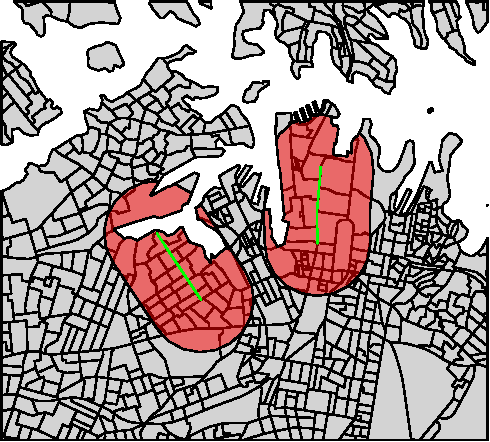
\includegraphics{catchmentplot-1} \caption[An 800 metre catchment area (red) associated with a cycle path (green) using straight-line distance in Sydney]{An 800 metre catchment area (red) associated with a cycle path (green) using straight-line distance in Sydney.}\label{fig:catchmentplot}
\end{figure}
\end{Schunk}

This simplistic catchment area is useful when the straight-line distance
is a reasonable approximation of the route taken to walk (or cycle) to a
transport facility. However, this is often not the case. The catchment
area in Figure \ref{fig:catchmentplot} initially appears reasonable but
the red-shaded catchment area includes an area that requires travelling
around a bay to access from the (green-coloured) cycleway. To allow for
more realistic catchment areas for most situations, \textbf{stplanr}
provides the \texttt{calc\_network\_catchment} function that uses the
same principle as \texttt{calc\_catchment} but also takes into account
the transport network.

To use \texttt{calc\_network\_catchment}, a transport network needs to
be prepared that can be used in conjunction with the previous datasets.
Preparation of the dataset involves using the
\texttt{SpatialLinesNetwork} function to create a network from a
\texttt{SpatialLinesDataFrame}. This function combines a
\texttt{SpatialLinesDataFrame} with a graph network (using the
\CRANpkg{igraph} package) to provide basic routing functionality. The
network is used to calculate the shortest actual paths within the
specific catchment distance. This process involves the following code:

\begin{Schunk}
\begin{Sinput}
unzip(file.path(data_dir, 'sydroads.zip'))
sydroads <- rgdal::readOGR(".", "roads")
file.remove(list.files(pattern = "^(roads).*"))
sydnetwork <- SpatialLinesNetwork(sydroads)
\end{Sinput}
\end{Schunk}

The network catchment is then calculated using a similar method as with
\texttt{calc\_catchment} but with a few minor changes. Specifically
these are including the \texttt{SpatialLinesNetwork}, and using the
\texttt{maximpedance} parameter to define the distance, with distance
being the additional distance from the network. In contrast to the
distance parameter that is based on the straight-line distance in both
the \texttt{calc\_catchment} and \texttt{calc\_network\_catchment}
functions, the \texttt{maximpedance} parameter is the maximum value in
the units of the network's weight attribute. In practice this is
generally distance in metres but can also be travel times, risk or other
measures.

\begin{Schunk}
\begin{Sinput}
netcatch800m <- calc_network_catchment(
  sln = sydnetwork,
  polygonlayer = sa1income,
  targetlayer = testcycleway,
  calccols = c('Total'),
  maximpedance = 800,
  distance = 100,
  projection = 'austalbers'
)
\end{Sinput}
\end{Schunk}

Once calculated, the network catchment area can be used just as the
straight-line network catchment. This includes extracting the catchment
population of 23457 and plotting the original catchment area together
with the original area with the results shown in Figure
\ref{fig:netcatchplot}:

\begin{Schunk}
\begin{Sinput}
plot(sa1income, col = "light grey")
plot(catch800m, col = rgb(1, 0, 0, 0.5), add = TRUE)
plot(netcatch800m, col = rgb(0, 0, 1, 0.5), add = TRUE)
plot(testcycleway, col = "green", add = TRUE)
\end{Sinput}
\begin{figure}
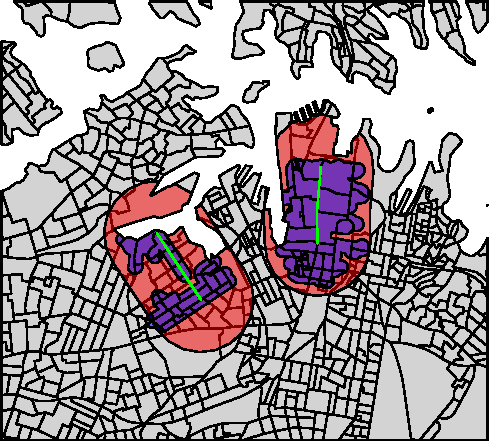
\includegraphics{netcatchplot-1} \caption[A 800 metre network catchment are (blue) compared with a catchment area based on Euclidean distance (red) associated with a cycle path (green)]{A 800 metre network catchment are (blue) compared with a catchment area based on Euclidean distance (red) associated with a cycle path (green).}\label{fig:netcatchplot}
\end{figure}
\end{Schunk}

\section{Modelling and visualisation}\label{modelling-and-visualisation}

\subsection{Modelling mode choice}\label{modelling-mode-choice}

Route-allocated lines allow estimation of \emph{route distance} and
\emph{cirquity} (route distance divided by Euclidean distance). These
variables can help model the rate of flow between origins and
destination, as illustrated in the left-hand panel of Figure
\ref{fig:euclidfastest}. The code below demonstrates how objects
generated by \textbf{stplanr} can be used to undertake such analysis,
with the \texttt{line\_length} function used to find the distance, in
meters, of lat/lon data.

\begin{verbatim}
l$d_euclidean <- line_length(l)
l$d_rf <- routes_fast@data$length
plot(l$d_euclidean, l$d_rf,
  xlab = "Euclidean distance", ylab = "Route distance")
abline(a = 0, b = 1)
abline(a = 0, b = 1.2, col = "green")
abline(a = 0, b = 1.5, col = "red")
\end{verbatim}

The left hand panel of Figure \ref{fig:euclidfastest} shows the expected
strong correlation between Euclidean (\(d_E\)) and fastest route
(\(d_{Rf}\)) distance. However, some OD pairs have a proportionally
higher route distance than others, as illustrated by distance from the
black line in the above plot: this represents \emph{Circuity ($Q$)}: the
ratio of network distance to Euclidean distance
\citep{levinson_minimum_2009}:

\[
 Q = \frac{d_{Rf}}{d_E}
\]

An extension to the concept of cirquity is the `quietness diversion
factor' (\(QDF\)) of a desire line \citep{lovelace_propensity_2016}, the
ratio of the route distance of a quiet route option (\(d_{Rq}\)) to that
of the fastest:

\[
 QDF = \frac{d_{Rq}}{d_{Rf}}
\]

Thanks to the `quietest' route option provided by
\texttt{route\_cyclestreet}, we can estimate average values for both
metrics as follows:

\begin{Schunk}
\begin{Sinput}
routes_slow <- line2route(l, route_cyclestreet, plan = "quietest")
\end{Sinput}
\end{Schunk}

\begin{Schunk}
\begin{Sinput}
l$d_rq <- routes_slow$length # quietest route distance
Q <- mean(l$d_rf / l$d_euclidean, na.rm = TRUE)
QDF <- mean(l$d_rq / l$d_rf, na.rm = TRUE)
Q
\end{Sinput}
\begin{Soutput}
#> [1] 1.298767
\end{Soutput}
\begin{Sinput}
QDF
\end{Sinput}
\begin{Soutput}
#> [1] 1.034721
\end{Soutput}
\end{Schunk}

The results show that cycle paths are not particularly direct in the
study region by international standards \citep{crow_design_2007}. This
is hardly surprisingly given the small size of the sample and the short
distances covered: \(Q\) tends to decrease at a decaying rate with
distance. What is surprising is that \(QDF\) is close to unity, which
could imply that the quiet routes are constructed along direct, and
therefore sensible routes. We should caution against such assumptions,
however: It is a small sample of desire lines and, when time is
explored, we find that the `quietness diversion factor with respect to
time' (\(QDF_t\)) is slightly larger:

\begin{Schunk}
\begin{Sinput}
(QDFt <- mean(routes_slow$time / routes_fast$time, na.rm = TRUE))
\end{Sinput}
\begin{Soutput}
#> [1] 1.052855
\end{Soutput}
\end{Schunk}

\subsection{Models of travel
behaviour}\label{models-of-travel-behaviour}

There are many ways of estimating flows between origins and
destinations, including spatial interaction models, the four-stage
transport model and gravity models (`distance decay'). \textbf{stplanr}
aims eventually to facilitate creation of many types of flow model.

At present there are no functions for modelling distance decay, but this
is something we would like to add in future versions of
\textbf{stplanr}. Distance decay is an especially important concept for
sustainable transport planning due to physical limitations on the
ability of people to walk and cycle large distances
\citep{iacono_measuring_2010}.

We can explore the relationship between distance and the proportion of
trips made by walking, using the same object \texttt{l} generated by
\textbf{stplanr}.

\begin{Schunk}
\begin{Sinput}
l$pwalk <- l$On.foot / l$All
plot(l$d_euclidean, l$pwalk, cex = l$All / 50,
  xlab = "Euclidean distance (m)", ylab = "Proportion of trips by foot")
\end{Sinput}
\end{Schunk}

\begin{Schunk}
\begin{figure}
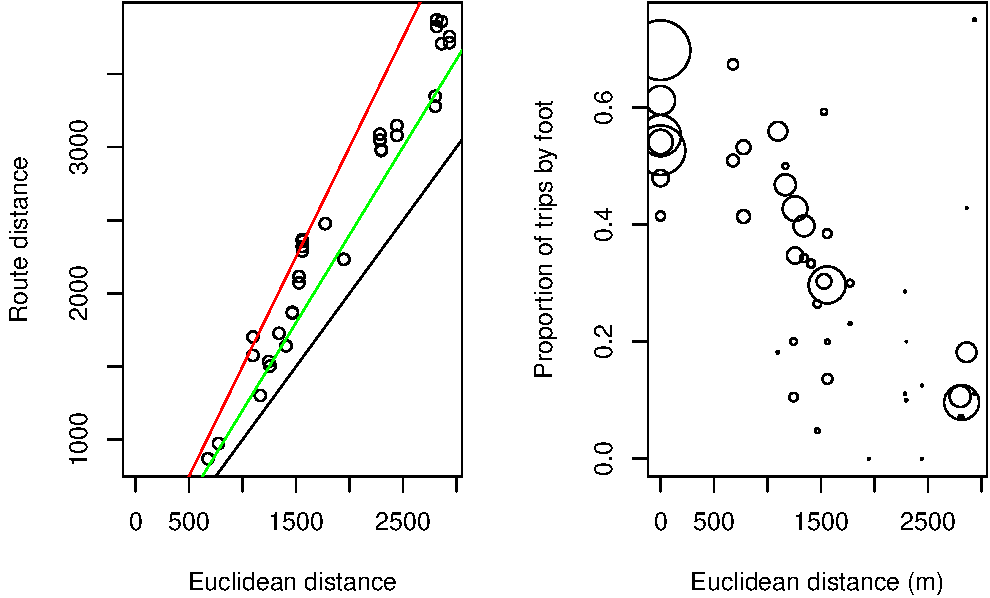
\includegraphics[width=1\linewidth]{euclidfastest-1} \caption[Euclidean and fastest route distance of trips in the study area (left) and Euclidean distance vs the proportion of trips made by walking (right)]{Euclidean and fastest route distance of trips in the study area (left) and Euclidean distance vs the proportion of trips made by walking (right).}\label{fig:euclidfastest}
\end{figure}
\end{Schunk}

Based on the right-hand panel in Figure \ref{fig:euclidfastest}, there
is a clear negative relationship between distance of trips and the
proportion of those trips made by walking. This is unsurprising: beyond
a certain distance (around 1.5km according the the data presented in the
figure above) walking is usually seen as too slow and other modes are
considered. According to the academic literature, this `distance decay'
is non-linear and there have been a number of functions proposed to fit
to distance decay curves \citep{martinez_new_2013}. From the range of
options we test below just two forms. We will compare the ability of
linear and log-square-root functions to fit the data contained in
\texttt{l} for walking.

\begin{Schunk}
\begin{Sinput}
lm1 <- lm(pwalk ~ d_euclidean, data = l@data, weights = All)
lm2 <- lm(pwalk ~ d_rf, data = l@data, weights = All)
lm3 <- glm(pwalk ~ d_rf + I(d_rf^0.5),
           data = l@data, weights = All, family = quasipoisson(link = "log"))
\end{Sinput}
\end{Schunk}

The results of these regression models can be seen using
\texttt{summary()}. Surprisingly, Euclidean distance was a better
predictor of walking than route distance, but no strong conclusions can
be drawn from this finding, with such a small sample of desire lines (n
= 42). The results are purely illustrative, of the kind of the
possibilities created by using \textbf{stplanr} in conjuction with R's
modelling capabilities (see Figure \vref{fig:euclidwalking2}).

\begin{Schunk}
\begin{Sinput}
plot(l$d_euclidean, l$pwalk, cex = l$All / 50,
  xlab = "Euclidean distance (m)", ylab = "Proportion of trips by foot")
l2 <- data.frame(d_euclidean = 1:5000, d_rf = 1:5000)
lm1p <- predict(lm1, l2)
lm2p <- predict(lm2, l2)
lm3p <- predict(lm3, l2)
lines(l2$d_euclidean, lm1p)
lines(l2$d_euclidean, exp(lm2p), col = "green")
lines(l2$d_euclidean, exp(lm3p), col = "red")
\end{Sinput}
\begin{figure}

{\centering 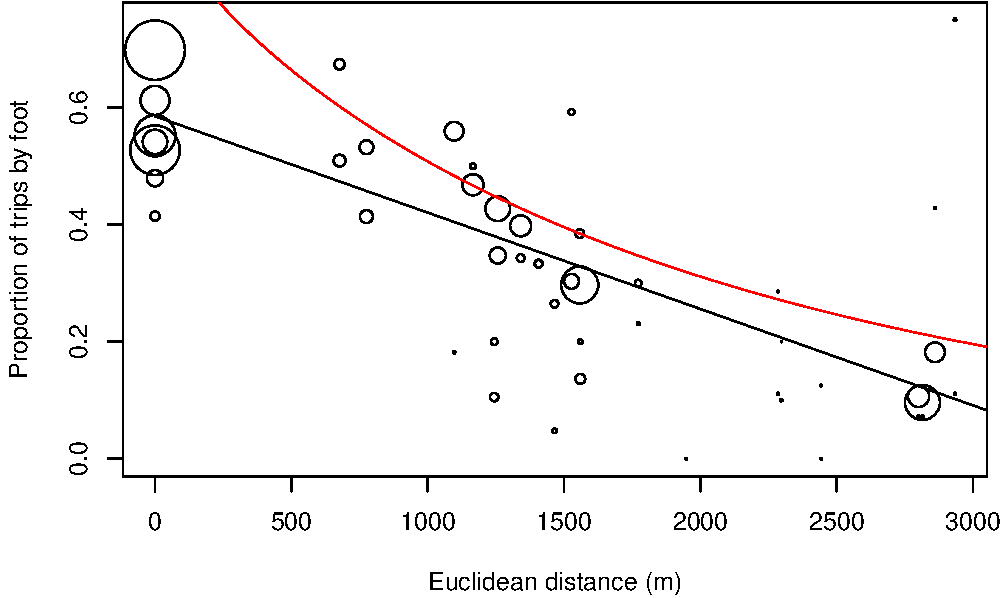
\includegraphics[width=0.75\linewidth]{euclidwalking2-1}

}

\caption[Relationship between euclidean distance and walking]{Relationship between euclidean distance and walking}\label{fig:euclidwalking2}
\end{figure}
\end{Schunk}

\subsection{Visualisation}\label{visualisation}

Visualisation is an important aspect of any transport study, as it
enables researchers to communicate their findings to other researchers,
policy-makers and, ultimately, the public. It may therefore come as a
surprise that \textbf{stplanr} contains no functions for visualisation.
Instead, users are encouraged to make use of existing spatial
visualisation tools in R, such as \textbf{tmap}, \textbf{leaflet} and
\textbf{ggmap} \citep{cheshire_spatial_2015,kahle_ggmap:_2013}.

Furthermore, with the development of online application frameworks such
as \textbf{shiny}, it is now easier than ever to make the results of
transport analysis and modelling projects available to the public. An
example is the online interface of the Propensity to Cycle Tool (PCT).
The results of the project, generated using \textbf{stplanr}, are
presented at zone, desire line and Route Network levels
\citep{lovelace_propensity_2016}. There is great potential to expand on
the principle of publicly accessible transport planning tools via `web
apps', perhaps through new R packages dedicated to visualising transport
data.

\section{Future directions of travel}\label{future-directions-of-travel}

This paper has demonstrated the great potential for R to be used for
transport planning. R's flexibility, powerful GIS capabilities
\citep{bivand_applied_2013} and free accessibility makes it well-suited
to the needs of transport planners and researchers, especially those
wanting to avoid the high costs of market-leading products. Rather than
`reinvent the wheel' (e.g.~with a new class system), \textbf{stplanr}
builds on existing packages and \CRANpkg{sp} classes to work with common
transport data formats.

It is useful to see \textbf{stplanr}, and R for transport planning in
general, as an addition tool in the transport planner's cabinet. It can
be understood as one part of a wider movement that is making transport
planning a more open and democratic process. Other developments in this
movement include the increasing availability of open data
\citep{naumova_building_2016} and the rise of open source products for
transport modelling, such as
\href{http://www.dlr.de/ts/en/desktopdefault.aspx/tabid-9883/16931_read-41000/}{SUMO},
\href{http://www.matsim.org/}{MATSim} and
\href{https://its.mit.edu/software/mitsimlab}{MITSIMLAB}
\citep{saidallah_comparative_2016}. \textbf{stplanr}, with its focus on
GIS operations rather than microscopic vehicle-level behaviour, can
complement such software and help make better use of new open data
sources.

Because transport planning is an inherently spatial activity,
\textbf{stplanr} occupies an important niche in the transport planning
software landscape, with its focus on spatial transport data. There is
great potential for development of \textbf{stplanr} in many directions.
Desirable developments include the additional of functions for modelling
modal split, for examample with functions to create commonly distance
decay curves which are commonly found in active travel research
\citep{martinez_new_2013} and improving the computational efficiency of
existing functions to make the methods more scalable for large
databases. Our priority for \textbf{stplanr} however, is to keep the
focus on geographic functions for transport planning. There are many
opportunities in this direction, including:

\begin{itemize}
\tightlist
\item
  Functions to assess the environment surrounding routes, e.g.~via
  integration with the in-development \textbf{osmdata} package.
\item
  Functions to match different GIS routes, perhaps building on the
  Hausdorf distance algorithm implemented in the \CRANpkg{rgeos}
  function \texttt{gDistance}.
\item
  Additional functions for route-allocation of travel, e.g.~via an
  interface to the OpenTripPlanner API.
\item
  Functions for aggregating very large GPS trace datasets (e.g.~into
  raster cells) for anonymisation and analysis/visualisation purposes.
\item
  The creation of a class system for spatial transport datasets, such as
  to represent spatial route and a route networks (perhaps with classes
  named \code{"sr"} and \code{"srn"}). This is not a short-term priority
  and it would be beneficial to coincide such developments to a
  migration to \CRANpkg{sf} for spatial classes.
\end{itemize}

Such spatial data processing capabilities would increase the range of
transport planning tasks that \textbf{stplanr} can facilitate. For all
this planned development activity to be useful, it is vital that new
functionality is intuitive. R has a famously steep learning curve.
Implementing simple concepts such as consistent naming systems
\citep{baath_state_2012} and ensuring `type stability' can greatly
improve the usability of the package. For this reason, much future work
in \textbf{stplanr} will go into improving documentation and
user-friendliness.

Like much open source software \textbf{stplanr} is an open-ended
project, a work-in-progress. We have set out clear motivations for
developing transport planning capabilities in R and believe that the
current version of \textbf{stplanr} (0.1.6) provides a major step in
that direction compared with what was available a couple of years ago.
But there is much more to do. We therefore welcome input on where the
package's priorities should lie, how it should evolve in the future and
how to ensure it is well-developed and sustained.

\bibliography{references}

\address{%
Robin Lovelace\\
University of Leeds\\
34-40 University Road\\ LS2 9JT, UK\\
}
\href{mailto:r.lovelace@leeds.ac.uk}{\nolinkurl{r.lovelace@leeds.ac.uk}}

\address{%
Richard Ellison\\
University of Sydney\\
378 Abercrombie Street\\ Darlington, NSW 2008, Australia\\
}
\href{mailto:richard.ellison@sydney.edu.au}{\nolinkurl{richard.ellison@sydney.edu.au}}

